\documentclass{article}
\usepackage[utf8]{inputenc}
\usepackage[margin=0.2in]{geometry}
\usepackage{graphicx}
\graphicspath{ {./images/} }
\usepackage{graphicx,wrapfig,lipsum}

\begin{document}
\twocolumn
{\Huge Alalisvool}\\
{\Large Saskia, nr4 2021}\\
Kirchhoffi I seadus e pingeseadus:
Kirchhoffi II seadus e vooluseadus:
\section{Stabiilsed ahelad}
\begin{center}
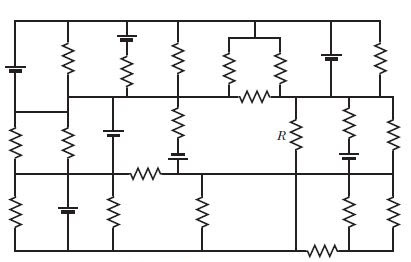
\includegraphics[width =  7cm]{ec2.jpg}
\end{center}
\subsection{Kondensaatorid}
\begin{center}
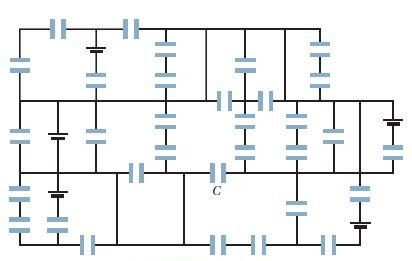
\includegraphics[width =  7cm]{ec1.jpg}
\end{center}
\section{Muutlikud vooluahelad}
\subsection{Dioodid}
\end{document}